\documentclass[../main.tex]{subfiles}
\graphicspath{{\subfix{../images/}}}

\begin{document}

Computers need to store data in order to function, like code, or data meaningful to you, like documents and images. Storage devices accomplish this. There are 3 main categories of storage devices, which will be covered here.

\subsection{RAM}
\label{3:sec:ram}

RAM or Random Access Memory; otherwise referred to as just Memory, stores \emph{volatile data} that does not have to be on your hard drive. It only stores data that the computer uses when it is on. Examples of data that goes into memory include temporary values that programs must store; from simple integers to browser tabs.

It has a property where it is directly addressable by the CPU. Check section \ref{3:sec:cpu} for details on exactly what that is, but it is essentially the brains of your computer. This makes RAM very fast.

\begin{figure}[H]
    \centering
    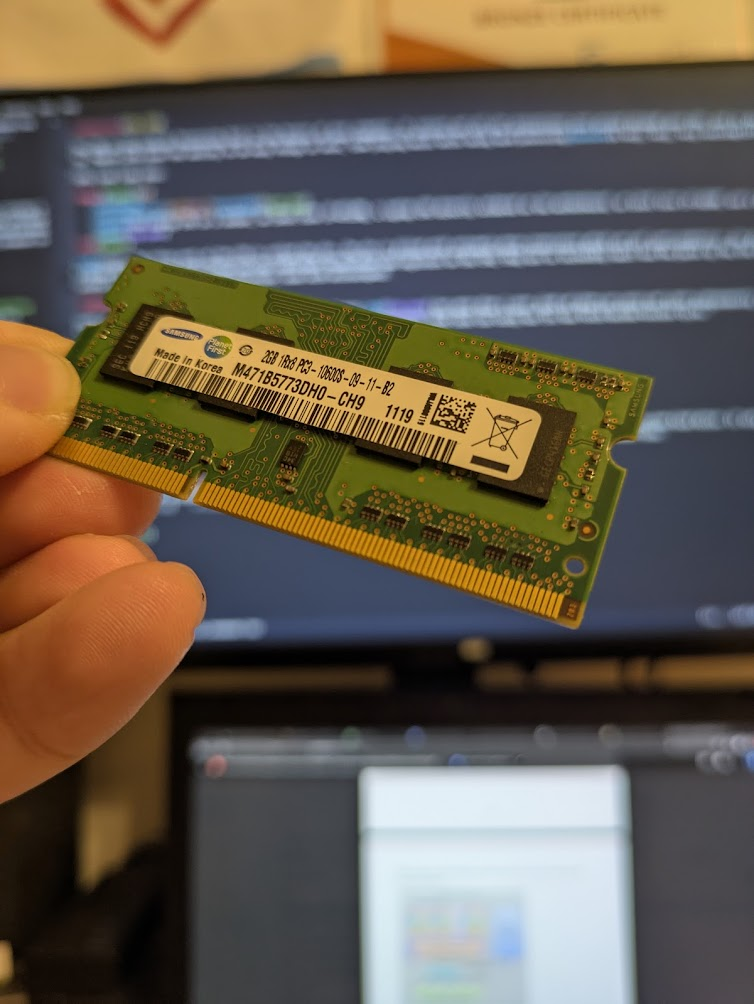
\includegraphics[width=0.5\textwidth]{ram.jpg}
    \caption{What a stick of LPDDR3 RAM (DRAM) looks like.}
    \label{fig:ram}
\end{figure}

Some important information include:

\begin{itemize}
    \item RAM can be freely written to, or read from. The data on RAM can be changed by the user, but not directly; through programs. As an example, opening a browser tab puts data into RAM, but you will not notice physical differences.
    \item RAM is \textbf{\emph{volatile}}. All data stored in it disappears when power to the RAM is lost.
    \item RAM is critical to your computer's function; as all code and data used by code is stored in RAM.
    \item Increasing the amount of RAM will boost the speed of your system, as the computer is able to store more of this temporary data at once in a fast location.
\end{itemize}

There are 2 main kinds of RAM, SRAM (S for static), and DRAM (D for dynamic).

\subsubsection{Dynamic RAM}

DRAM chips (the black squares that you see on the image) consist of transistors and capacitors. It is by far the most common type of RAM in all computers. The access time for DRAM is \textasciitilde60 milliseconds.

They consist of:

\begin{itemize}
    \item Capacitors hold a bit of information (0, or 1)
    \item Transistors act as switches, which allows the chip's control circuitry to read or write to the capacitors.
\end{itemize}

This must be constantly refreshed, as the capacitors cannot hold data for very long.

Benefits of DRAM include:

\begin{itemize}
    \item Much cheaper to make than SRAM
    \item Consume less power on average
    \item They hold a larger total capacity (typically)
    \item DRAM in computers are upgradable in many cases. Modern laptops do not allow you to do so for the most part, but all desktops and some older laptops allow you to remove and exchange DRAM easily for upgrades/repairs.
\end{itemize}

Drawbacks of DRAM include:

\begin{itemize}
    \item It needs constant refreshing to keep the capacitors charged
    \item It is slower than SRAM, by more than 2 times. This limits its applications.
\end{itemize}

\subsubsection{Static RAM}

SRAM chips are made of flip-flops that hold a constant one bit value. They do not need to be constantly refreshed, therefore. SRAM is used when speed is required, such as the CPU's cache. The access time is \textasciitilde25 milliseconds.

Benefits of SRAM include:

\begin{itemize}
    \item Much faster than DRAM due to less latency\footnote{Delay.}
    \item Consumes less power
    \item Does not need to be constantly refreshed
\end{itemize}

Drawbacks of SRAM include:

\begin{itemize}
    \item Much more expensive
    \item Very low capacity
    \item More complex and typically incompatible circuitry must be used to access the RAM.
\end{itemize}

\subsubsection{Differences between DRAM and SRAM}

\begin{longtable}{|p{0.4\textwidth}|p{0.4\textwidth}|}
    \hline 
    \textbf{Dynamic RAM (DRAM)} & \textbf{Static RAM (SRAM)}
    \\ \hline
    DRAM is slower & SRAM is faster
    \\ \hline
    Uses transistors to control the flow of electrons, and capacitors store the binary 1s and 0s & Uses flip-flop circuits
    \\ \hline
    Must be constantly refreshed to make sure the capacitors have charge & Does not need refreshing
    \\ \hline
    Cheaper to make & Much more expensive to make
    \\ \hline
    In a computer, the main memory uses it & The CPU's cache uses it
    \\ \hline
    Less overall power consumption & More overall power consumption
    \\ \hline
    Higher capacity & Lower capacity
    \\ \hline
\end{longtable}

\subsection{ROM}

ROM is like RAM, however, it stands for \emph{read-only memory.} Like RAM (see section \ref{3:sec:ram}), it stores data that is quickly accessible to the computer; i.e. directly addressible by the CPU. However, the \emph{key difference} is that \textbf{ROM is NOT erased when the computer powers off.} This is part of the reason why ROM is purely read-only. ROM cannot be erased.\footnote{Nowadays, computers do not use pure ROM chips anymore, as...they cannot be erased. Instead, they use EEPROM, or electrically-erasable and programmable ROM, which can be erased, but not as easily as RAM. You need a special device to erase an EEPROM, but it is doable. This means that manufacturing errors when making ROM can just be overwritten.}

The main use of ROM in computers is to store the BIOS/UEFI. This is code that the CPU executes immediately when the computer starts up. It does critical checks to make sure all your peripherals are working (like your keyboard), applies specific security patches to your CPU that the CPU maker sees fit, and loads the OS (see section \label{4:sec:the_os_and_kernel}. Increasing the size of ROM does nothing in most systems.

\subsection{Virtual Memory}

\subsection{HDDs (Hard disk drives)}

\subsection{SSDs (Solid state drives)}

\subsection{USB Mass Storage (Flash Drives)}

\subsection{Optical Media}

\subsection{QR Codes}

\end{document}
